\renewcommand{\captiontitle}{\UNet{} 模块}
\begin{figure}
\centering
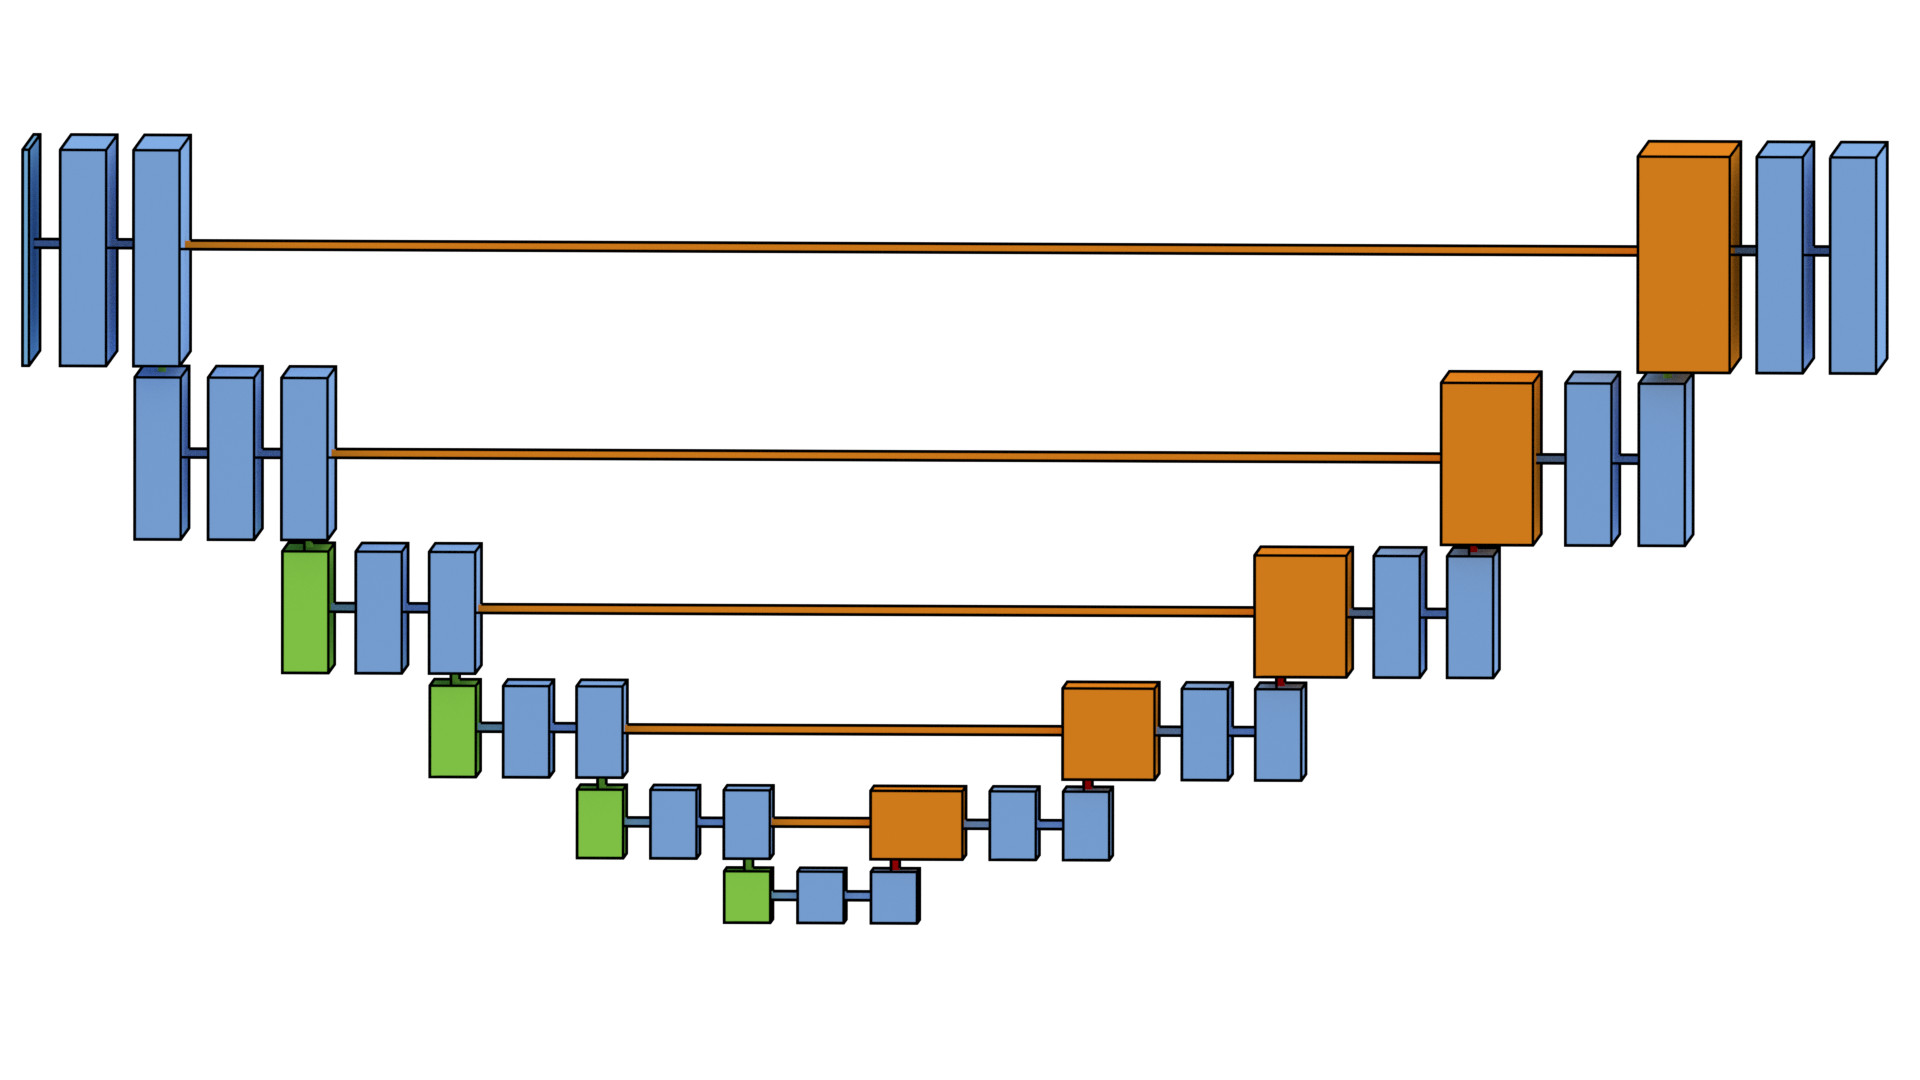
\includegraphics[clip, trim=0 0 0 0,width=0.5\textwidth]{./data/unet-module.png}
\caption[\captiontitle]{\captiontitle{}.  输入图像尺寸为 $\N \times \N \times N$,其中 $N$ 通道数(所有网络的通道数均为 $1$).
蓝色、绿色和橙色方框对应着多通道的特征图.绿色对应的是下采样的特征图,橙色对应的是将结果与特征图的拼接.}
\label{fig:unet-module}
\end{figure}

